\newpage
\section{Initializing a table: \addbs{tkzTabInit}}
\subsection{Definition}

\begin{NewMacroBox}{tkzTabinit}%
{\oarg{local options}\var{e(1)/h(1),...,e(p)/h(p)}\var{a(1),...,a(n)}}

\begin{tabular}{lllc}
\toprule
arguments &  default  & definition                 \\
\midrule
\TAline{list1} {no default }  {\var{e(1)/h(1),...,e(p)/h(p)} }
\TAline{list2} {no default }  {\var{a(1),...,a(n)}}
\bottomrule
\end{tabular}

\medskip
\noindent\emph{The mandatory arguments of this macro are two comma-separated lists. The first one has $p$ elements, which define $p$ rows of the table. The second one has $n$ elements, which define $n$ values of the variable. Each value of the variable corresponds to a column.}

 \begin{itemize}

\item List 1: \emph{the elements of the first list are pairs \tkzname{e(i)/h(i)}, where \tkzname{/} separates an expression \tkzname{e(i)} from a number expressed in \tkzname{centimeters}. For every $i$, \tkzname{h(i)} is a decimal number: the height in \tkzname{cm} of the row that contains the expression \tkzname{e(i)}. Decimal numbers use a period as decimal separator.}

\item List 2: \emph{the symbols ``\tkzname{/}'' and ``\tkzname{,}'' cannot be used in \tkzname{e(i)} unless they are protected inside a group\protect\footnotemark. Instead of protecting a comma with a pair of braces, as in |\{4,5\}|, you can use a command such as \tkzcname{numprint\{4,5\}} or \tkzcname{np\{4,5\}}\protect\footnotemark.}
 \end{itemize}
\NamePack{numprint}

\medskip
\begin{tabular}{lllc}
\toprule
options             & default & definition                         \\
\midrule
\TOline{espcl}  {3 cm}{space between two values                     }
\TOline{lgt}     { 2 cm}{width of the first column                  }
\TOline{deltacl}{0.5 cm}{margin before the first and after the last value}
\TOline{lw}    {0.4 pt}{line width of the table                     }
\TOline{nocadre}{false}{by default, the table is framed              }
\TOline{color} {false}{boolean, allows colors\protect\footnotemark}
\TOline{colorC} {white}{color of the first column                   }
\TOline{colorL} {white}{color of the first row                      }
\TOline{colorT} {white}{color of the main part                      }
\TOline{colorV} {white}{color of the cell of the variable           }
\TOline{help}   {false}{shows the names of the construction points  }  \bottomrule
\end{tabular}

\medskip
\noindent\emph{The table above describes the current options of the macro. The first three are essential for the appearance of your table and for its final size. You can also use the options of the \tkzname{tikzpicture} environment: \tkzname{scale}, \tkzname{xscale} and \tkzname{yscale}.}
\end{NewMacroBox}

% three \footnotemark in the box: number the texts from the first mark
\addtocounter{footnote}{-2}\footnotetext{an expression between braces.}
\stepcounter{footnote}\footnotetext{See the documentation of the package \tkzname{numprint}.}
\stepcounter{footnote}\footnotetext{It is better to load the package \tkzname{xcolor} with options such as \tkzname{usenames} or \tkzname{dvipsnames}.}

\subsection{Using the arguments}
\subsubsection{A simple table}
\medskip
Example: \begin{tkzexample}[code only]\tikz \tkzTabInit{$x$ /.8 , $f(x)$ /.8}{$0$ , $+\infty$}; \end{tkzexample}creates a table with \tkzname{two} rows. Each row is $\np{0.8}$ cm high. The bounds of the right column are $0$ and $+\infty$.

\medskip
\begin{center}
  \tikz \tkzTabInit{$x$ /.8 , $f(x)$ /.8}{$0$ , $+\infty$};
\end{center}
\subsubsection{Adding rows and columns}

The first list gives three rows, each $1$ cm high. The second list has three values of the variable, which define two intervals (zones). Vertical rules can be drawn below these values.

\begin{tkzexample}[width=10cm,small]
\begin{tikzpicture}
\tkzTabInit
 {$x$      /1,
  $f(x)$   /1,
  $g(x)$   /1}
 {$0$,$\E$,$+\infty$}
\end{tikzpicture}
\end{tkzexample}
Note the use of the macro \tkzcname{E} \footnote{\tkzcname{E} is defined by \BS newcommand*\{\BS E\}\{\BS ensuremath\{\BS mathrm\{e\}\}\}.}
\subsubsection{Minimal table}
\index{Minimal table}
The first argument is \tkzname{ /1}: this is the minimal argument. The argument is a list whose separator is the symbol \tkzname{/}, preceded here by a space or by nothing, so the first cell of the row is empty. \tkzname{$1$} means \tkzname{$1$ cm}: a dimension in cm is required to give the height of the row. The second argument is made of two empty elements, or of two spaces separated by a comma. This argument must contain at least two elements: the bounds of an interval.

\begin{tkzexample}[width=8cm,small]
\begin{tikzpicture}
 \tkzTabInit{  / 1}
            {  ,  }
\end{tikzpicture}
\end{tkzexample}

\subsection{Using the options}

First, some dimensions of the columns can be changed. Here are the default values.

\begin{center}
  \begin{tikzpicture}
     \tkzTabInit
        {$x$ /  1}
        {$a_1$ ,  $a_2$ , $a_3$}
    \begin{scope}[arstyle/.style={>=latex,#1,<->}]
      \draw[arstyle=blue] (N10) to node[above,color=blue]%
           {\scriptsize $ espcl = 3$ cm} (N20);
      \draw[arstyle=blue] (N20) to node[above,color=blue]%
           {\scriptsize $ espcl = 3$ cm} (N30);
      \draw[arstyle=red] (T10) to node[above=12pt,color=red]%
           {\scriptsize $ deltacl = 0.5$ cm} (N10);
      \draw[arstyle=red] (N30) to node[above=12pt,color=red]%
           {\scriptsize $ deltacl = 0.5$ cm} (T20);
      \draw[arstyle=blue] (T00) to node[above,color=blue]%
           {\scriptsize $ lgt = 2$ cm} (T10);
    \end{scope}
  \end{tikzpicture}
\end{center}


\subsubsection{\texttt{\textcolor{red}{lgt}}: width of the first column}\Iopt{tkzTabInit}{lgt}

By default, the first column is $2$ cm wide. The unit is always the \tkzname{cm}.

\begin{tkzexample}[width=8cm,small]
\begin{tikzpicture}
  \tkzTabInit[lgt=3]{ $x$ / 1}
                    { $1$  , $3$ }
\end{tikzpicture}
\end{tkzexample}

\subsubsection{\texttt{\textcolor{red}{espcl}}: space between two values}\Iopt{tkzTabInit}{espcl}

\begin{tkzexample}[width=9cm,small]
\begin{tikzpicture}
   \tkzTabInit[lgt=3,espcl=4]%
    { $x$ / 1}
    { $1$ , $4$  }
\end{tikzpicture}
\end{tkzexample}

\subsubsection{\texttt{\textcolor{red}{deltacl}}: margins at both ends}\Iopt{tkzTabInit}{deltacl}

\begin{tkzexample}[width=9cm,small]
\begin{tikzpicture}
  \tkzTabInit[lgt=3,deltacl=1]%
  { $x$ / 1}
  { $1$ , $4$ }
\end{tikzpicture}
\end{tkzexample}

\subsubsection{\texttt{\textcolor{red}{lw}}: line width of the table}
\Iopt{tkzTabInit}{lw}
This is not recommended: all the lines of a document should preferably have the same width, which is $\np{0.4}$ pt by default.

\begin{tkzexample}[width=8cm,small]
\begin{tikzpicture}
  \tkzTabInit[lw=2pt]{ / 1}
                    { , }
\end{tikzpicture}
\end{tkzexample}

\subsubsection{\texttt{\textcolor{red}{nocadre}}: removing the outer frame}
\Iopt{tkzTabInit}{nocadre}

\begin{tkzexample}[width=8cm,small]
\begin{tikzpicture}
  \tkzTabInit[nocadre]{ / 1, /1, /1}
                      { , }
\end{tikzpicture}
\end{tkzexample}

\subsubsection{\texttt{\textcolor{red}{color}}: using colors in a table}
\Iopt{tkzTabInit}{color}\NamePack{amsmath}
\tkzname{color} is a boolean that says you want to use colors. You then give the colors of the first row \tkzname{colorL}, of the first column \tkzname{colorC}, of the cell of the variable \tkzname{colorV} and of the rows \tkzname{colorT}. A color can also be given to a particular row.

\tkzname{tkzTabInit\{[color]\}} means that the boolean color is true.

\begin{tkzexample}[width=8cm,small]
\begin{tikzpicture}
  \tkzTabInit[color,
              colorT = yellow!20,
              colorC = orange!20,
              colorL = green!20,
              colorV = lightgray!20]
             { /1 , /1}{ , }
\end{tikzpicture}
\end{tkzexample}

\begin{tkzexample}[width=8cm]
\begin{tikzpicture}
 \tkzTabInit[color,
             colorT = yellow!20,
             colorC = red!20,
             colorL = green!20,
             colorV = lightgray!20,
             lgt    = 1,
             espcl  = 2.5]%
   {$t$/1,$a$/1,$b$/1,$c$/1,$d$/1}%
   {$\alpha$,$\beta$,$\gamma$}%
\end{tikzpicture}
\end{tkzexample}

\subsubsection{\texttt{\textcolor{red}{help}}: shows the structure of the table}
\Iopt{tkzTabInit}{help}
See the section ``Customizing the tables'' (\ref{pers}).
\endinput
